\part{Calcul numérique et discret}\index{Calcul numérique et discret}
\chapter{Nombres à virgule flottante}\index{Nombres à virgule flottante}
Dans les chapitres suivants, les nombres à virgule flottante sont au cœur des
calculs ; il convient de les étudier car leur comportement suit des règles précises.
Comment représenter des nombres réels en machine ? Comme ces nombres ne
peuvent pas en général être codés avec une quantité finie d’information, ils ne
sont pas toujours représentables sur un ordinateur : il faut donc les approcher
avec une quantité de mémoire finie.
Un standard s’est dégagé autour d’une approximation des nombres réels avec
une quantité fixe d’information : la représentation à virgule flottante.
Dans ce chapitre, on trouve : une description sommaire des nombres à virgule
flottante et des différents types de ces nombres disponibles dans SymPy, et la 
démonstration de quelques-unes de leurs propriétés. Quelques exemples montreront
certaines des difficultés qu’on rencontre en calculant avec les nombres à virgule
flottante, quelques astuces pour arriver parfois à les contourner, en espérant 
développer chez le lecteur une prudence bien nécessaire ; en conclusion, nous essayons
de donner quelques propriétés que doivent posséder les méthodes numériques pour
pouvoir être utilisées avec ces nombres.

\chapter{Intégration numérique}\index{Intégration numérique}
Ce chapitre traite le calcul numérique d’intégrales (§14.1) ainsi que la résolution
numérique d'équations différentielles ordinaires (§14.2) avec SymPy. Nous rappelons
des bases théoriques des méthodes d’intégration, puis nous détaillons les fonctions
disponibles et leur usage (§14.1.1). Le calcul symbolique d’intégrales avec SymPy a été traité précédemment (§2.3.8), et ne sera que mentionné rapidement ici comme une possibilité de calculer la
valeur numérique d’une intégrale. Cette approche « symbolique puis numérique »,
lorsqu’elle est possible, constitue une des forces de SymPy et est à privilégier car le
nombre de calculs effectués, et donc d’erreurs d’arrondi, est en général moindre
que pour les méthodes d’intégration numérique. Nous donnons une rapide introduction aux méthodes classiques de résolution d’équations différentielles, puis le traitement d’un exemple (§14.2.1) débutera l’inventaire des fonctions disponibles en SymPy (§14.2.2).

On s’intéresse au calcul numérique d’intégrales de fonctions réelles ; pour une
fonction $f : I \longrightarrow R$, où $I$ est un intervalle de $\mathbb{R}$, on veut calculer :
\[
\int_{I} f\left(x\right).
\]

Par exemple, calculons
\[
 \int_{1}^{3} x^{2}e^{-x^{2}}\cos\left(x\right) dx.
\] 

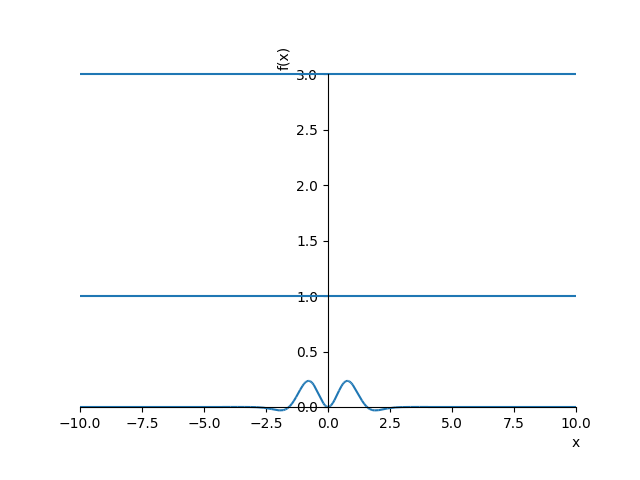
\includegraphics[scale=0.6]{../Pictures/Figure_1.png} 
\begin{python}
from sympy.abc import x
from sympy import integrate
from sympy.plotting import plot
f = x**2*exp(-x**2)*cos(x)
N(integrate(f, (x, 1, 3))
0.0306905101632536
plot(f, (1, 3, fill='axis'))
\end{python}

La fonction integrate calcule l’intégrale symbolique de l’expression, il faut
demander explicitement une valeur numérique pour l’obtenir.
\\
Il est aussi, en principe, possible de calculer des intégrales sur un intervalle
dont les bornes sont infinies :
\begin{python}
from sympy.abc import x
from sympy import sin, oo
N(integrate(sin(x**2)/(x**2), (x, 1, oo))
0.285736646322853
plot(sin(x**2)/(x**2), x, 1, 10, fill='axis')
\end{python}

\subsection{Equation and Text}\index{Examples!Equation and Text}

\begin{example}
Let $G=\{x\in\mathbb{R}^2:|x|<3\}$ and denoted by: $x^0=(1,1)$; consider the function:
\begin{equation}
f(x)=\left\{\begin{aligned} & \mathrm{e}^{|x|} & & \text{si $|x-x^0|\leq 1/2$}\\
& 0 & & \text{si $|x-x^0|> 1/2$}\end{aligned}\right.
\end{equation}
The function $f$ has bounded support, we can take $A=\{x\in\mathbb{R}^2:|x-x^0|\leq 1/2+\epsilon\}$ for all $\epsilon\in\intoo{0}{5/2-\sqrt{2}}$.
\end{example}

\chapter{Transformation d'intégrale}
 \section{Transformation de Fourier}
 \begin{exercise}
 \end{exercise}
 \begin{exercise}
 \end{exercise}
 \begin{exercise}
 \end{exercise}
  \subsection{Transformation de Fourier inverse}
  \begin{exercise}
 \end{exercise}
 \begin{exercise}
 \end{exercise}
 \section{Transformation de Laplace}
 \begin{python}
 \end{python}
 \begin{exercise}
 \end{exercise}
 \section{Transformation de Mellin}
 \begin{example}
  La transformée d'une distribution de Dirac ${\displaystyle \delta (x-a)}$, avec $a > 0$, est une fonction exponentielle ${\displaystyle s\mapsto a^{s-1}}$.
 \end{example}
 \begin{python}
 \end{python}
 \begin{example}
  La transformée de Mellin de la fonction ${\displaystyle f\,:\,x\mapsto \mathrm {H} (a-x)} {\displaystyle f\,:\,x\mapsto \mathrm {H} (a-x)}$, avec $a > 0$, est la fonction ${\displaystyle s\mapsto {\frac {a^{s}}{s}}} {\displaystyle s\mapsto {\frac {a^{s}}{s}}}$ sur le demi-plan $Re (s) > 0$
(où $H$ est la fonction de Heaviside, $f(x) = 1$ si $0 < x < a et f (x) = 0 si x > a$).
 \end{example}
 \begin{python}
 \end{python}
 \begin{example}
%   La transformée de Mellin de la fonction ${\frac {1}{\mathrm {e} ^{x}-1}}}$ est la fonction ${\displaystyle s\mapsto \Gamma (s)\zeta (s)}$ sur le demi-plan $Re (s) > 1$
 \end{example}
 \begin{python}
 \end{python}
 \subsection{Transformation de melin inverse}
 \section{Transfomation de Henkel}
 La transformée de Hankel (d'ordre zéro) est une transformée intégrale équivalente à une transformée de Fourier à deux dimensions avec un noyau intégral à symétrie radiale, appelée également transformation de Fourier-Bessel. Il est défini comme
 \[
 g \left(u, v \right)	= F_{r}\left[\left(r\right)\right]\left(u, v\right)
 \]
 \subsection{Transformation de Henkel inverse}
 
\chapter{Équations non linéaires}\index{Équations non linéaires}
Ce chapitre explique comment résoudre une équation non linéaire avec SymPy.
Dans un premier temps on étudie les équations polynomiales et on montre les
limitations de la recherche de solutions exactes. Ensuite on décrit le fonctionnement
de quelques méthodes classiques de résolution numérique. Au passage on indique
quels sont les algorithmes de résolution numérique implémentés dans SymPy.
Qu'est ce que non-linéaire et qu'est ce que une \'equation alg\'ebrique

Une \'equation alg\'ebrique est un polyn\^ome de la forme $P(x)$

\begin{equation}
\exp(-x)\sin(x) = \cos(x)
\end{equation}
\section{Équations algébriques}